\begin{figure}[p]\centering
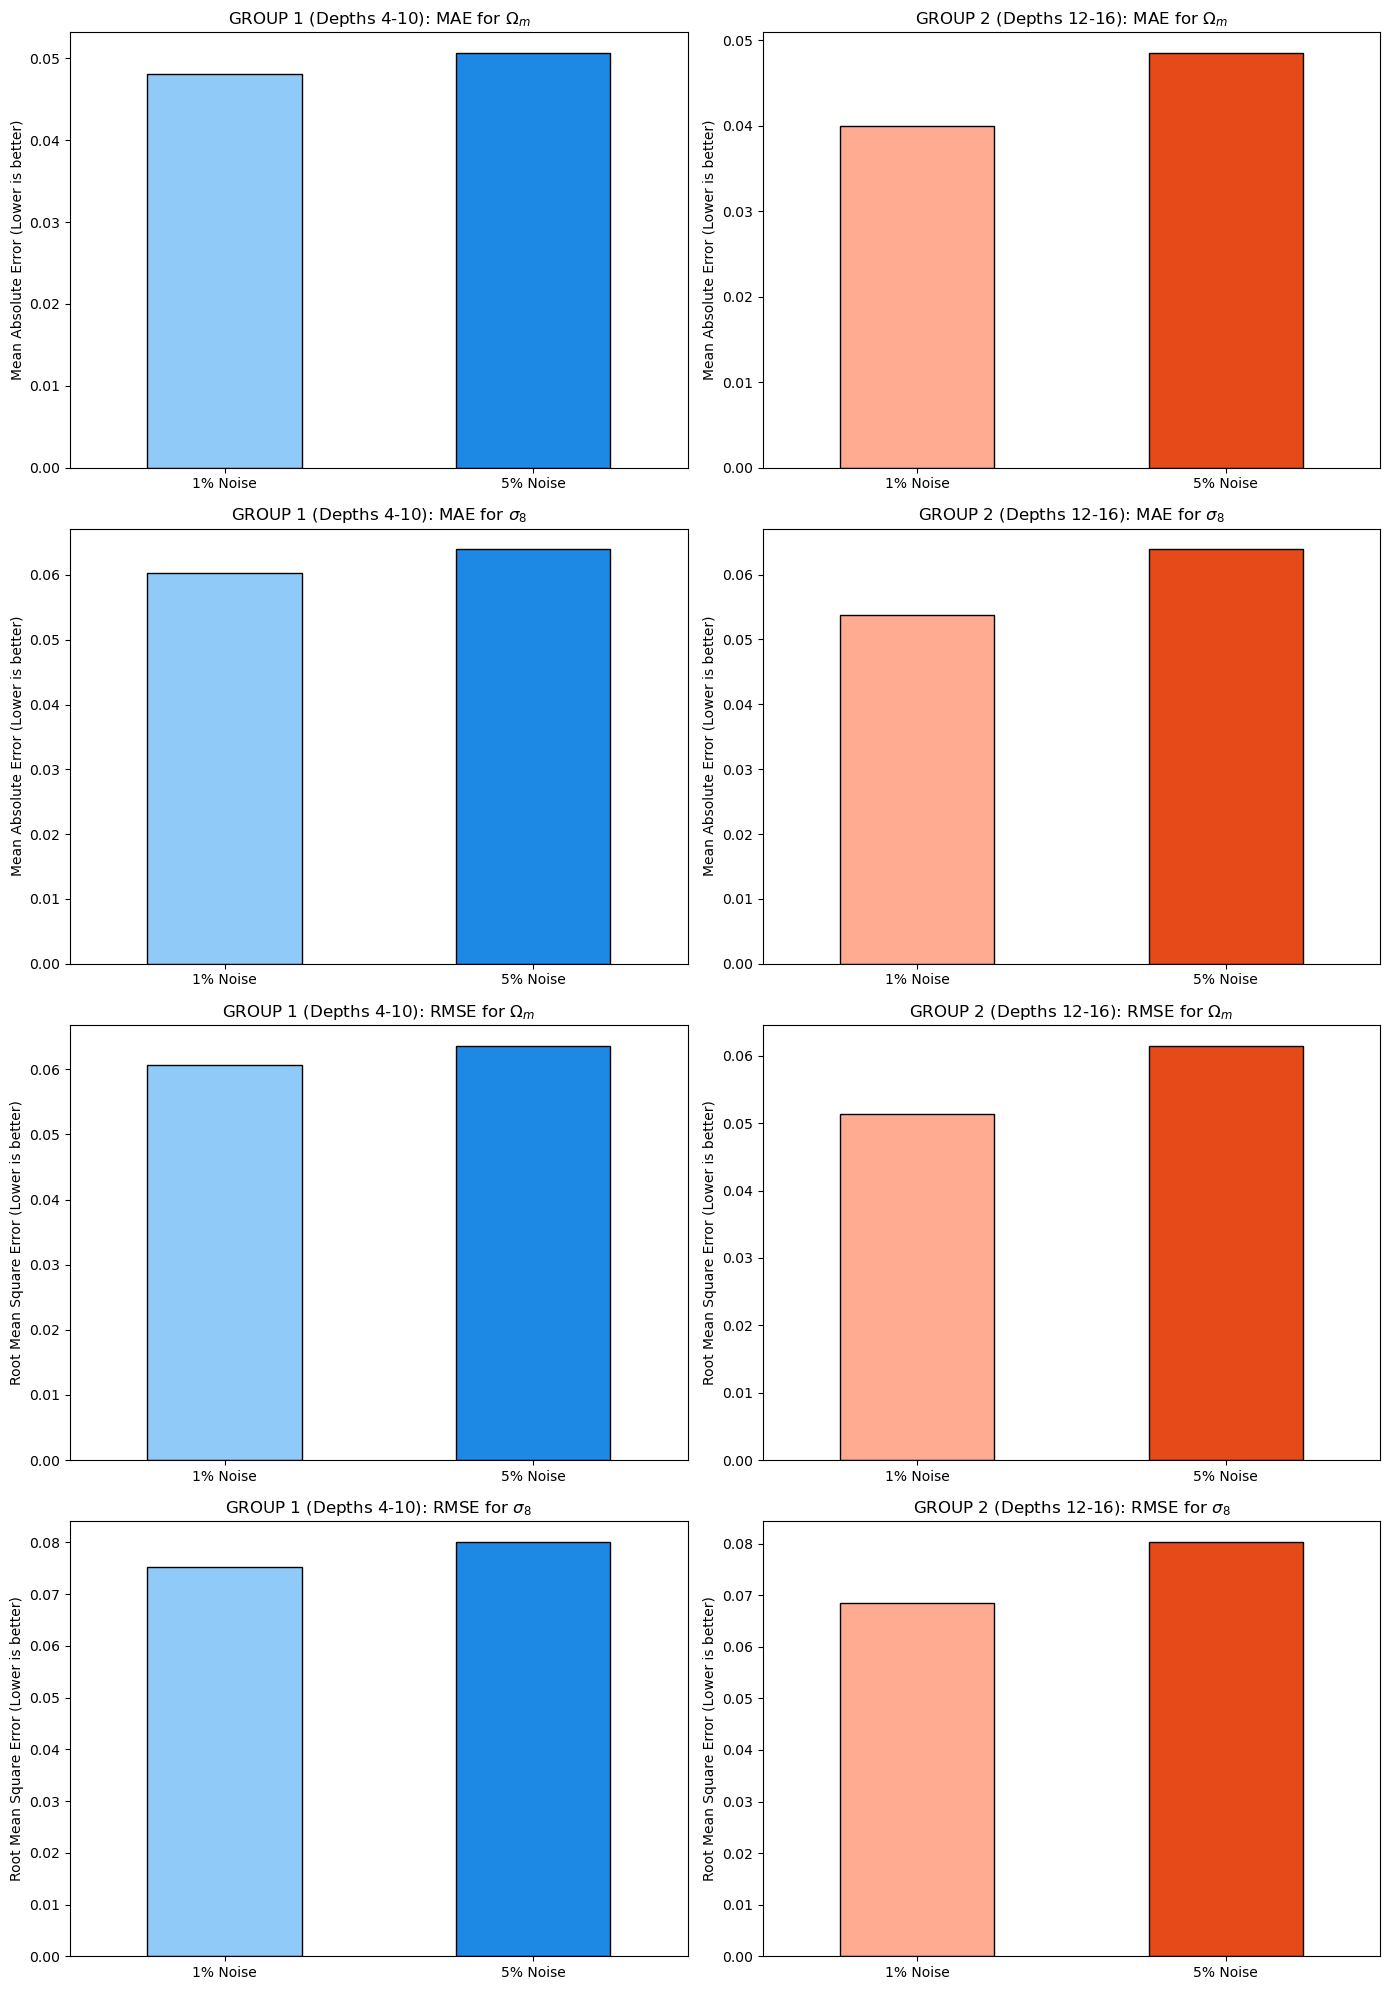
\includegraphics[width=.92\linewidth,height=.72\textheight,keepaspectratio]{figures/nb_compare_results_c3_o0.png}
\caption{Embedded notebook rendering from \texttt{augment/compare\_results.ipynb}, cell 3 (zero based). This preserves the notebook's saved version of the plot.}
\end{figure}\clearpage
\begin{figure}[p]\centering
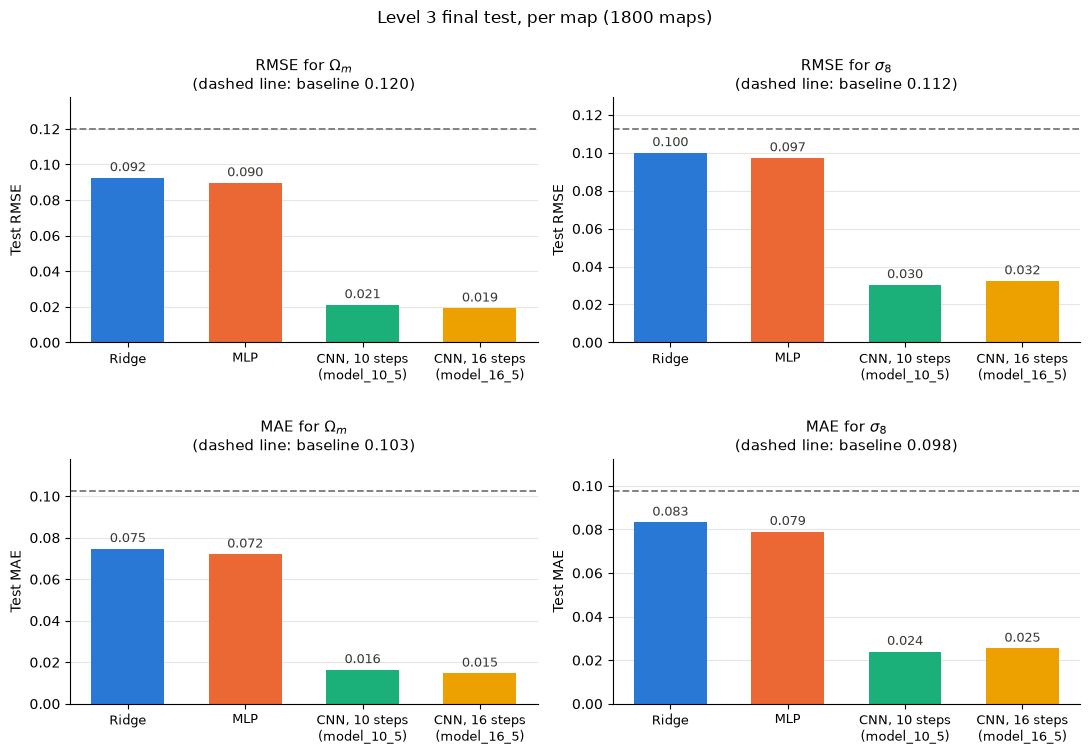
\includegraphics[width=.92\linewidth,height=.72\textheight,keepaspectratio]{figures/nb_cnn_test_c12_o0.png}
\caption{Embedded notebook rendering from \texttt{cnn\_test/cnn\_test.ipynb}, cell 12 (zero based). This preserves the notebook's saved version of the plot.}
\end{figure}\clearpage
\begin{figure}[p]\centering
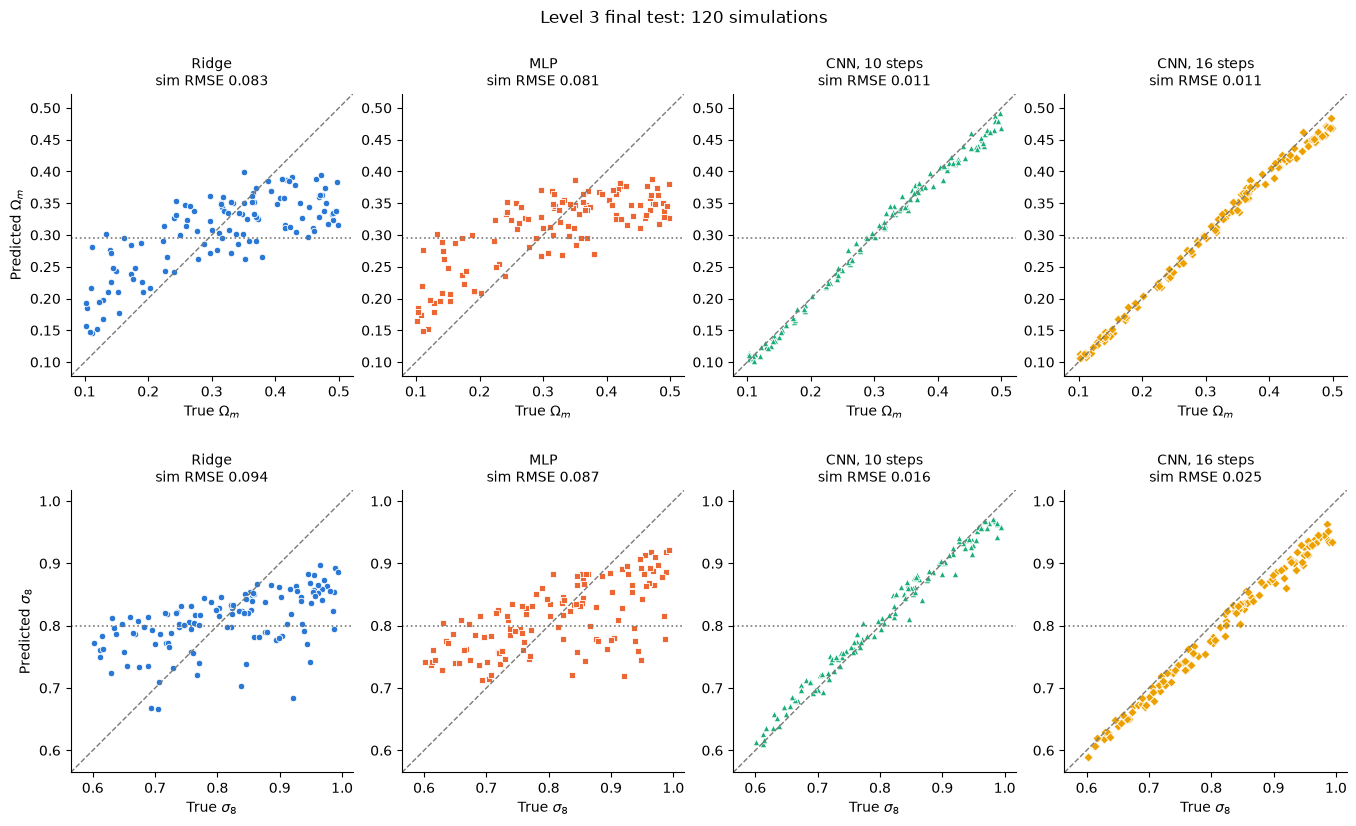
\includegraphics[width=.92\linewidth,height=.72\textheight,keepaspectratio]{figures/nb_cnn_test_c14_o0.png}
\caption{Embedded notebook rendering from \texttt{cnn\_test/cnn\_test.ipynb}, cell 14 (zero based). This preserves the notebook's saved version of the plot.}
\end{figure}\clearpage
\begin{figure}[p]\centering
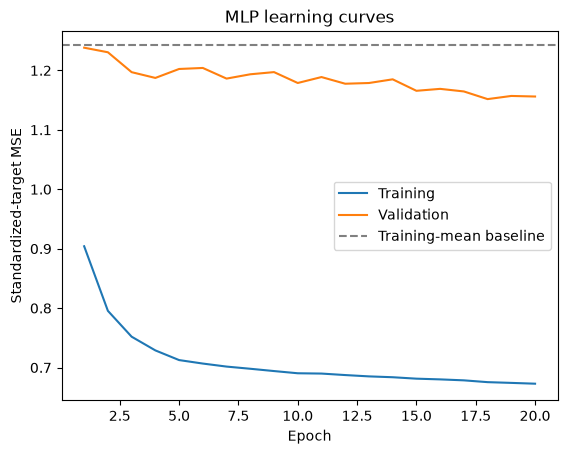
\includegraphics[width=.92\linewidth,height=.72\textheight,keepaspectratio]{figures/nb_mlp_validation_c28_o0.png}
\caption{Embedded notebook rendering from \texttt{mlp/level1/mlp\_validation.ipynb}, cell 28 (zero based). This preserves the notebook's saved version of the plot.}
\end{figure}\clearpage
\begin{figure}[p]\centering
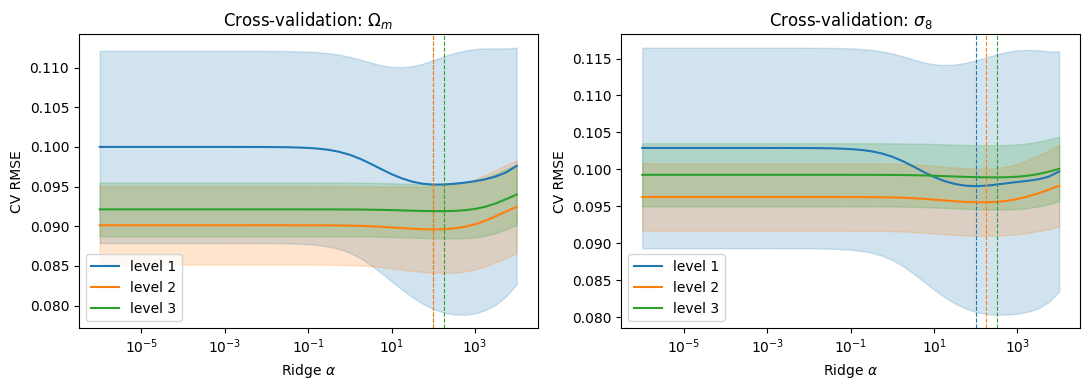
\includegraphics[width=.92\linewidth,height=.72\textheight,keepaspectratio]{figures/nb_ridge_c8_o0.png}
\caption{Embedded notebook rendering from \texttt{ridge.ipynb}, cell 8 (zero based). This preserves the notebook's saved version of the plot.}
\end{figure}\clearpage
\begin{figure}[p]\centering
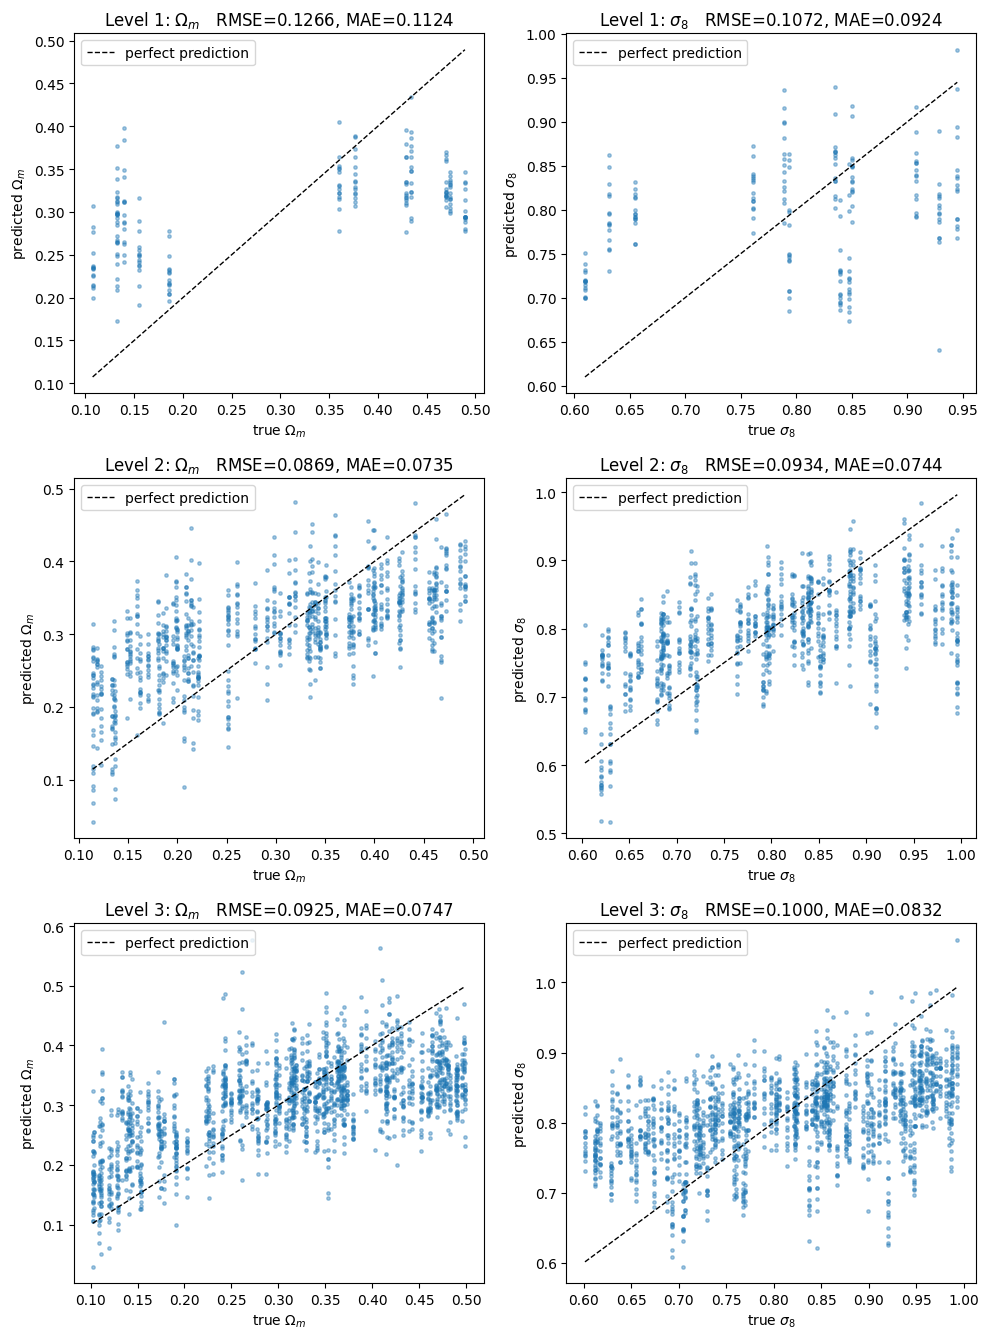
\includegraphics[width=.92\linewidth,height=.72\textheight,keepaspectratio]{figures/nb_ridge_c11_o0.png}
\caption{Embedded notebook rendering from \texttt{ridge.ipynb}, cell 11 (zero based). This preserves the notebook's saved version of the plot.}
\end{figure}\clearpage
\begin{figure}[p]\centering
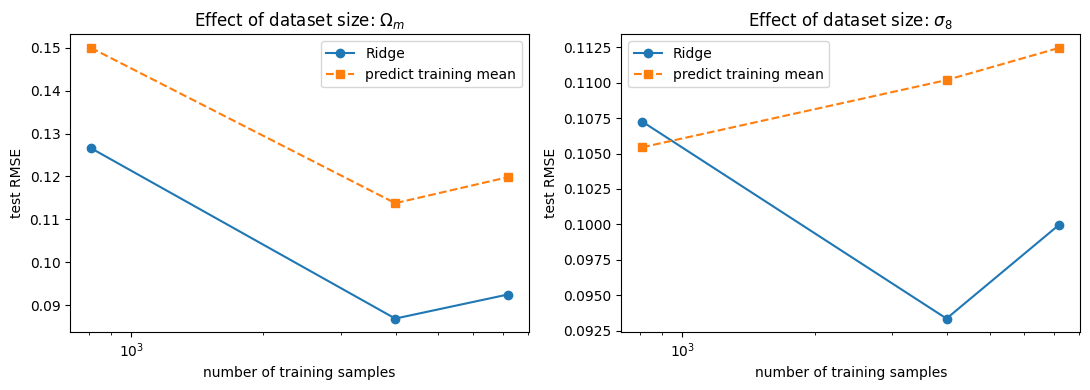
\includegraphics[width=.92\linewidth,height=.72\textheight,keepaspectratio]{figures/nb_ridge_c12_o0.png}
\caption{Embedded notebook rendering from \texttt{ridge.ipynb}, cell 12 (zero based). This preserves the notebook's saved version of the plot.}
\end{figure}\clearpage